%%%%%%%%%%%%%%%%%%%%%%%%%%%%%%%%%%%%%%%%%%%%%%%%%%%%%%%%%%%%%%%%%%%%
% PREAMBLE
%%%%%%%%%%%%%%%%%%%%%%%%%%%%%%%%%%%%%%%%%%%%%%%%%%%%%%%%%%%%%%%%%%%%%
%
% The following two commands will generate a PDF that follows all the requirements for submission
% and peer review.  Uncomment these commands to generate this output (and comment out the two lines below.)
%
% DOUBLE SPACE VERSION FOR SUBMISSION TO THE AMS
%\documentclass[12pt]{article}
\documentclass[10pt]{article}
\usepackage{ametsoc}
%\usepackage{ametsoc2col}
\linenumbers

% Ryan's custom commands
\newcommand{\pd}[2]{ \frac{\partial #1}{\partial #2} }
\newcommand{\od}[2]{\ensuremath{\frac{d #1}{d #2}}}
\newcommand{\td}[2]{\ensuremath{\frac{D #1}{D #2}}}
\newcommand{\ab}[1]{\ensuremath{\langle #1 \rangle}}
\newcommand{\bss}[1]{\textsf{\textbf{#1}}}
\newcommand{\ol}{\ensuremath{\overline}}
\newcommand{\olx}[1]{\ensuremath{\overline{#1}^x}}
\newcommand{\nms}{\ensuremath{\mbox{ N m}^{-2}}}
\newcommand{\wmm}{\ensuremath{\mbox{ W m}^{-2}}}
\newcommand{\mms}{\ensuremath{\mbox{ m}^2 \mbox{ s}^{-1}}}
\newcommand{\mss}{\ensuremath{\mbox{ m s}^{-2}}}
\newcommand{\ihat}{\hat{\textbf{\i}}}
\newcommand{\jhat}{\hat{\textbf{\j}}}
\newcommand{\orho}{\frac{1}{\rho_0}}

%
% The following two commands will generate a single space, double column paper that closely
% matches an AMS journal page.  Uncomment these commands to generate this output (and comment
% out the two lines above. FOR AUTHOR USE ONLY. PAPERS SUBMITTED IN THIS FORMAT WILL BE RETURNED
% TO THE AUTHOR for submission with the correct formatting.
%
% TWO COLUMN JOURNAL PAGE LAYOUT FOR AUTHOR USE ONLY
%%%%\documentclass[10pt]{article}
%%%%\usepackage{ametsoc2col}
%
%%%%%%%%%%%%%%%%%%%%%%%%%%%%%%%%%%%%%%%%%%%%%%%%%%%%%%%%%%%%%%%%%%%%%
% ABSTRACT
%
% Enter your Abstract here
%%%%%%%%%%%%%%%%%%%%%%%%%%%%%%%%%%%%%%%%%%%%%%%%%%%%%%%%%%%%%%%%%%%%%
\newcommand{\myabstract}{Blah.}
%
\begin{document}
%
%%%%%%%%%%%%%%%%%%%%%%%%%%%%%%%%%%%%%%%%%%%%%%%%%%%%%%%%%%%%%%%%%%%%%
% TITLE
%
% Enter your TITLE here
%%%%%%%%%%%%%%%%%%%%%%%%%%%%%%%%%%%%%%%%%%%%%%%%%%%%%%%%%%%%%%%%%%%%%
\title{\textbf{\large{Phase Speed Cross Spectra of Eddy Heat Fluxes in the Pacific}}}
%
% Author names, with corresponding author information. 
% [Update and move the \thanks{...} block as appropriate.]
%
\author{\textsc{Ryan Abernathey}
				\thanks{\textit{Corresponding author address:} 
				Ryan Abernathey, Lamont-Doherty Earth Observatory, 
				Palisades, NY. 
				\newline{E-mail: rpa@ldeo.columbia.edu}}\\
\textit{\footnotesize{Columbia University, New York, New York}}
\and 
\centerline{\textsc{Cimarron Wortham}}\\% Add additional authors, different institution
\centerline{\textit{\footnotesize{Applied Physics Laboratory, University of Washington, Seattle, Washington}}}
}
%
% Formatting done here...Authors should skip over this.  See above for abstract.
\ifthenelse{\boolean{dc}}
{
\twocolumn[
\begin{@twocolumnfalse}
\amstitle

% Start Abstract (Enter your Abstract above.  Do not enter any text here)
\begin{center}
\begin{minipage}{13.0cm}
\begin{abstract}
	\myabstract
	\newline
	\begin{center}
		\rule{38mm}{0.2mm}
	\end{center}
\end{abstract}
\end{minipage}
\end{center}
\end{@twocolumnfalse}
]
}
{
\amstitle

\begin{abstract}
\myabstract
\end{abstract}

\newpage
}

%%%%%%%%%%%%%%%%%%%%%%%%%%%%%%%%%%%%%%%%%%%%%%%%%%%%%%%%%%%%%%%%%%%%%
% MAIN BODY OF PAPER
%%%%%%%%%%%%%%%%%%%%%%%%%%%%%%%%%%%%%%%%%%%%%%%%%%%%%%%%%%%%%%%%%%%%%
\section{Introduction}

Transient motions (a.k.a.~``eddies'') in the ocean and atmosphere lead to significant material transport. Of particular importance is the meridional eddy heat transport, which contributes to the maintenance of Earth's pole-to-equator temperature gradient \citep{TrenberthCaron2001,Wunsch2005}. Although eddy heat fluxes in the ocean are relatively less significant than in the atmosphere, they are still an important part of the ocean heat budget, particularly at regional scales and in the Southern Ocean \citep{JayneMarotzke2002,WhatElse?}. Because of their small spatial scales, ocean eddy fluxes are more difficult or observe than those in the atmosphere, and their statistical properties are less well characterized. Satellites provide a uniquely powerful tool for observing eddies at the ocean surface. Climate models are also beginning to resolve the ocean mesoscale.

A fundamental question is what determines the strength of the eddy flux and how this flux is related to more readily observable eddy properties such as eddy size, kinetic energy, etc.
%A further, more challenging question is whether this flux can be parameterized in terms of large scale hydrographic properties; this problem is theoretically interesting but also practically relevant for ocean general circulation models (GCMs), which do not resolve eddies and therefore must parameterize their effects. 
Inspired by the classical ``mixing length'' arguments of \citet{Taylor1915} and \citet{Prandtl1925} regarding turbulent fluxes, many studies have assumed the eddy flux in the ocean to be proportional to the background tracer gradient (i.e.~that it is diffusive) and to the product of a characteristic eddy size and eddy velocity \citep[e.g.][]{Holloway1986,KefferHolloway1988,VisbeckEtAl1997,Stammer1998}. More recent studies have added a new ingredient to the equation: the eddy phase speed, i.e.~the eddy propagation relative to the background mean flow \citep{MarshallEtAl2006,SmithMarshall2009,AbernatheyEtAl2010,FerrariNikurashin2010,KlockerEtAl2012a,KlockerEtAl2012b,AbernatheyMarshall2013}. In particular, the simple stochastic model of \citet{FerrariNikurashin2010} demonstrates how zonal phase propagation suppresses meridional eddy diffusion and puts forth a quantitative theory for the magnitude of this effect.

The framework of \citet{FerrariNikurashin2010} was recently tested by \citet[][henceforth KA14]{KlockerAbernathey2014} in a comprehensive way using kinematic tracer simulations in the east Pacific (the same sector studied here). Those results indicate that the extratropical meridional eddy flux of a passive tracer due to mesoscale eddy stirring could be parameterized quite well in terms of a single wavenumber and phase speed at each latitude. The appropriate phase speed is the long baroclinic Rossby wave phase speed, while the appropriate wavenumber is proportional to the average diameter of tracked nonlinear coherent eddies from the eddy census of \citet{CheltonEtAl2011}. The fact that the eddy flux can be parameterized in terms of an essentially monochromatic model seems at odds with the fact that the ocean contains a broad spectrum of variability in space and time \citep{WorthamWunsch2014}. Therefore, a key motivation for our study is to attempt to reconcile the success of the monochromatic FN10 model with the broadband nature of the variability. We wish to asses how narrowly concentrated the eddy flux is around a single length scale and phase speed.

To answer this question, we employ satellite observations to investigate the spectral character of surface eddy meridional heat fluxes over a wide range of latitudes. This is achieved by calculating wavenumber-frequency cross-spectra for sea-surface temperature (SST) and the geostrophic velocity derived from sea-surface height (SSH). There is an extensive literature on the analysis of spatiotemporal variance and covariance in different remotely sensed ocean surface datasets such as SSH, SST, and color-derived chlorophyl \citep[see review by][]{OBrienEtAl2013}. Many of these past studies focus on characterizing the propagation behavior of Rossby waves \citep{CheltonSchalx1996,PolitoCornillon1997,CipolliniEtAl1997,HillEtAl2000,CipolliniEtAl2001,PolitoLiu2003,KillworthEtAl2004} and tropical instability waves \citep{PolitoEtAl2001,Contreras2002,CheltonEtAl2000,LeeEtAl2012}. The paper by \citet{KillworthEtAl2004} is particularly comprehensive and makes a convincing case that a large fraction of of the variance in SST and surface chlorophyl arises by advective stirring by the surface geostrophic flow by motions propagating close to the long Rossby wave speed.

Being interested in the wave dynamics themselves, the studies cited above generally employed filters to isolate the spectral bands of interest. Here the approach is slightly different: we consider the total, unfiltered eddy flux and examine its spectral density in wavenumber, frequency, and phase-speed space. This perspective is inspired by the atmospheric study of \citet[][henceforth RH91]{RandelHeld1991}, who made such a diagnosis for the eddy fluxes of heat and momentum in the troposphere. In particular, presenting the results of the cross-spectral analysis through 2D contour plots as a function of latitude and phase speed (or latitude and wavenumber) provides a novel view of the oceanographic data, revealing the strong latitudinal dependence in the spectra. Our results indicate that the extratropical meridional eddy heat flux in phase-speed space is indeed concentrated around the long Rossby-wave phase speed\footnote{One slightly confusing yet well documented fact to keep in mind is  that coherent nonlinear eddies propagate at this phase speed, but larger (apparently linear) Rossby waves propagate somewhat faster \citep{CheltonEtAl2007,CheltonEtAl2011}.}. Furthermore, the dominant length scale associated with the eddy heat flux is everywhere very close to the observed mesoscale eddy diameter. These conclusions help to explain the success of KA14.

In addition to analyzing the satellite data, we perform the same analysis on a state-of-the-art global eddy-resolving / eddy-permitting ocean model. This comparison serves two purposes. On one hand, it allows us probe finer space and time scales than the observations can resolve. On the other, it provides a form of model validation in the spectral domain. The broad agreement between the model and the observations is encouraging on both fronts, suggesting that the observations are more than sufficient to resolve the dominant scales of eddy heat transport and that the model shares the spectral characteristics of the observations.

%Finally, to probe the physics that give rise to the observed spectra, we analyze kinematic simulations of advective stirring of the climatological SST pattern by satellite-derived velocity fields.

Our paper is organized as follows. Sec.~2 describes the satellite data sources used for SST and SSH. The basic results of the cross-spectral analysis are presented in Sec.~3 as function of latitude and wavenumber, latitude and frequency, and latitude and phase speed. In Sec.~4, we diagnose the moments of the flux and its ``breadth'' in wavenumber and phase-speed space. We also compare the total flux to the prediction of the FN10 model. Discussion and conclusions are given in Sec.~5.

%%%%%%%%%%%%%%%%%%%%%%%%%%%%%%%%%%%%%%%%%%%%%%%%%%%%%%%%%%%%%%%%%%%%%
% Data
%%%%%%%%%%%%%%%%%%%%%%%%%%%%%%%%%%%%%%%%%%%%%%%%%%%%%%%%%%%%%%%%%%%%%
\section{Data and Models}

We focus our study on a sector in the east Pacific ranging from 180$^\circ$ to 130$^\circ$W in longitude and spanning 60$^\circ$S to 50$^\circ$N longitude. Beyond the intrinsic importance of the eastern Pacific for global climate variability (for example, related to the El Ni\~no / Southern Oscillation phenomenon), this sector was chosen specifically to facilitate comparison between our results and those of KA14 and \citet{AbernatheyMarshall2013}. Those earlier works picked this sector because it is relatively statically homogeneous in longitude and contains very little land. These attributes are also well suited to our purposes here, which is to examine the dependence of the spectra on latitude. Understanding the spectral character of eddy fluxes in more inhomogeneous regions, such as western boundary currents, is an important problem but beyond the scope of this work.

\subsection{Sea-Surface Height (SSH)}
Sea surface height data is used to estimate surface geostrophic velocities. The altimeter products were produced by SSALTO/DUACS and distributed by AVISO, with support from CNES (\url{http://www.aviso.oceanobs.com/duacs/}). For this study we use the pre-computed geostrophic velocities derived from the delayed-time, two-satellite ``reference" merged sea-level anomaly fields . In these pre-computed velocities, the method of \citet{LagerloefEtAl1999} is applied in the equatorial band ($\pm 5^\circ$). This method, based on the ``equatorial geostrophic'' vorticity balance, has been validated with {\em in situ} current meters and allows us to obtain velocity estimates in this region. Nevertheless, we must maintain some skepticism of the results in the equatorial band;  we focus primarily on the extra tropics.

The horizontal spacing of the AVISO gridded data is 1/4$^\circ$. The effective resolution of the product is such that it ``sees'' eddies of approx.~50 km diameter and larger \citep{CheltonEtAl2011}; however, smoothing is applied during the gridding procedure acts as a low-pass filter, attenuating the signal weakly at wavelengths below 200 km and strongly below 100 km \citep{DucetEtAl2000}. Consequently, the SSH signal displays very little power at short wavelengths (see Fig.~\ref{fig:integrated_spectra_V}). This filtering would make it difficult to estimate, for example, spectral slopes characterizing turbulent inertial ranges from the gridded data \citep{XuFu2011}. However, the focus here is not on the inertial range but of the prominent peak wherein most of the kinetic energy resides. This peak, which is everywhere at wavelengths larger than 200 km, is well resolved by the gridded data; mixing-length arguments suggest that these large-scale, highly energetic motions should also dominate the heat flux. Directly assessing the contribution of the filtered smaller scales to the heat flux could potentially be explored using along-track data, but we do not take that route here. However, one motivation for examining the numerical model (with 1/10$^\circ$ resolution, described below) is to attempt to probe smaller scales. In both model and data, we find the heat flux is dominated by wavelengths larger than 200 km.

Aviso produces a map every 7 days which represents a best estimate of the SSH field on that day. The data record begins in 1992, but we only consider the 9.3 year period concurrent with the SST observations, as described below.

\subsection{Sea-Surface Temperature (SST)}

The SST data is the Group for High Resolution Sea Surface Temperature (GHRSST) global Level 4 sea surface temperature analysis produced by the NOAA National Climatic Data Center \citep{ReynoldsEtAl2007}. An SST map is produced daily on a 1/4$^\circ$ grid. We selected the version of the product that blends data from the 4-km Advanced Very High Resolution Radiometer (AVHRR), the Advanced Microwave Scanning Radiometer-EOS (AMSR-E), and {\em in situ} ship and buoy observations using optimal interpolation. The SST value represents the temperature at approx.~0.3 m depth. The data coverage for this product begins in June 2002 and ends in Oct. 2011, the period of operation of the AMSR-E instrument. In order to match the temporal resolution of the SSH data, we subsample the SST data on the same days as the Aviso output.

\subsection{1/10$^\circ$ POP Model}

The model analyzed here, a version of the Community Climate System Model (CCSM), is described in \citet{MccleanEtAl2011}.  (The CCSM code name for this run is {\tt 	hybrid\_v5\_rel04\_BC5\_ne120\_t12\_pop62}.) This is a global climate simulation which includes ocean, atmosphere, sea-ice, and land models. The ocean component, our focus here, uses the Parallel Ocean Program (POP) code and is henceforth referred to as the ``POP model.'' The POP model has a nominal grid spacing of 0.1$^\circ$ and the atmosphere 0.25$^\circ$. The two are coupled every six hours. This combination of high-resolution atmosphere, ocean, and coupling results in one of the most realistic global simulations currently available. We consider the use of a coupled model (rather than an ocean-only model) important for simulating the complex air-sea interactions that arise over mesoscale eddies \citep{SmallEtAl2008,BryanEtAl2010}, which may influence the eddy heat flux.

We extract daily surface velocity and SST fields from the same sector described above for a five year period (model years 46-50). This is significantly higher temporal resolution than the AVISO data. While higher frequency motions are clearly present in the model spectra, our analysis below indicates that these high frequency (super-weekly) components make a negligible contribution to the meridional heat flux.

Note that we do not attempt to isolate the geostrophic component of the flow in the model; while this would allow for a more direct comparison with the AVISO results, we prefer instead to examine the full eddy flux produced by the model. As we will see, the similarity between the model and satellite results suggests that the flux in the model is indeed dominated by geostrophic motions.

\subsection{Pre-Processing}

Relatively little additional processing is applied to the data, since the observational products we have chosen are already highly processed. We subtract the time mean at each point in space (this is already done in the case of AVISO fields, which are the anomaly relative to 1993-1999 mean), and then the zonal mean at each time step, effectively removing the seasonal cycle and the basin-scale variability. Everything remaining is included in our definition of ``eddy'' variability.

\subsection{Coherent Eddy Statistics}

A large amount of the variance in midlatitude SSH has been attributed to coherent, nonlinear mesoscale eddies \citep{CheltonEtAl2011}. Throughout this study, we compare the length scales and phase speeds that arise from our spectral analysis with the coherent eddy characteristics from the eddy census of \citet{CheltonEtAl2011}, whose results were made publicly available\footnote{{\tt http://cioss.coas.oregonstate.edu/eddies/}}. The observed eddy length scale $L_s$ is defined by the average radius of all the eddies at each latitude in the sector. This radius itself is determined for each eddy from the area enclosed by the SSH contour corresponding to the maximum geostrophic flow speed, i.e.~where the eddy velocity is greatest. (See \citealt{CheltonEtAl2011}, Sec.~4.2 for further discussion of the eddy length computation.) To convert this length scale to a wavenumber, we follow the recommendation of \citet{CheltonEtAl2011} and assume the eddy streamfunction to be described by a gaussian function with an $e$-folding scale of $\sqrt{2} L_s$. We then define the corresponding eddy wavenumber as $K_{eddy} = (\sqrt{2} L_s)^{-1}$.

Two additional length scales are relevant to our study. The first baroclinic Rossby radius of deformation is a fundamental length scale for the dynamics of large-scale ocean circulation; of particular relevance here is the fact that the most unstable mode of baroclinic instability occurs near the deformation radius \citep{CheltonEtAl1998,Stammer1998,Smith2007}. It is also enters into the Rossby wave dispersion relation. Following \citet{TullochEtAl2009} (whose deformation radius data we borrowed), the first baroclinic deformation wavenumber is defined as the largest eigenvalue $K_d$ given by the Sturm-Liouville equation
\begin{equation}
\od{}{z}\left (\frac{f^2}{N^2} \od{\Phi}{z} \right ) = - K_d^2 \Phi
\end{equation}
where $f$ is the Coriolis parameter and $N$ is the Brunt--V{\"a}is{\"a}l{\"a} frequency. Our $K_d$ values represent a zonal average over the sector. Given $K_d$, the long baroclinic Rossby wave phase speed in the zonal direction is then given by
\begin{equation}
c_R = \ol{U}^{zt}  - \beta K_d^{-2}
\label{eq:c_R}
\end{equation}
where $\ol{U}^{zt}$ is the time- and depth-averaged zonal flow (a Doppler-shift term) and $\beta$ is the meridional gradient of $f$. As shown by KA14, $c_R \simeq c_{eddy}$ in this sector. We also invoke the Rhines scale, defined as the wavenumber $K_\beta = (\beta / 2 u_{rms} )^{1/2}$, where $u_{rms}$ is the root-mean-square eddy velocity (calculated from the AVISO data). This represents the scale at which turbulent motions become effective at transferring energy into zonally elongated flow such as jets \citep{Rhines1975,VallisMaltrud1993}.

For a given wavenumber $K$, the wavelength is defined as $L = 2 \pi / K$. While elementary, this conversion can be a source of great confusion. For example, under this terminology  the Rossby deformation {\em wavelength} near 45 S is approx.~120 km (as in \citealt{TullochEtAl2009}); this is greater than the deformation {\em radius} of \citet{CheltonEtAl1998} by a factor of $2 \pi$. It is common to plot wavenumber spectra in terms of ``cycles per meter,'' which implies the division of wavenumber $K$ by a factor of $2 \pi$. This quantity is best described as an ``inverse wavelength,'' not a wavenumber. Correct treatment of this issue is crucial, for example, in assessing the strength of the inverse cascade.


%\subsection{Issues}
%\begin{itemize}
%\item Aliasing: by sampling the data every 7 days, we are potentially aliasing high frequency signals. How can this be minimized?
%\item Windowing: should we be using a window in space or in time?
%\item Errors: how do we propagate / estimate errors in these spectra.
%\item Could we be using multi-taper instead of straight FFT?
%\end{itemize}

%%%%%%%%%%%%%%%%%%%%%%%%%%%%%%%%%%%%%%%%%%%%%%%%%%%%%%%%%%%%%%%%%%%%%
% DFT
%%%%%%%%%%%%%%%%%%%%%%%%%%%%%%%%%%%%%%%%%%%%%%%%%%%%%%%%%%%%%%%%%%%%%
\section{Cross-Spectral Analysis}

Here we describe the technical details of the spectral analysis and present the basic results. Extensive discussion of the results is deferred until Sec.~4.

\subsection{Univariate Power Spectra for SST and Surface Meridional Velocity}

Here we describe the calculation of wavenumber-frequency spectra for $\theta$, the SST. (An identical procedure applies to $v$, the meridional velocity.) In principle, $\theta$ is a continuous function of $x$, zonal coordinate, and $t$, time: $\theta = \theta(x,t)$ at each latitude $\varphi$ in the sector. However, our observations are discrete, with $N$ spatial points in longitude (spaced by $\Delta x$) and $M$ points in time (spaced by $\Delta t$) such that the total zonal length of the sector is $L = N \Delta x$ and the total temporal length of the record is $T = M \Delta t$. The discrete space and time coordinates are denoted as $x_n = n \Delta x$, $t_m = m \Delta t$. For the satellite data used here, $L(\varphi) = 2 \pi a \cos(\varphi) (50/360)$ where $\varphi$ is latitude, $N = 200$, $T = 3402$ days, and $M = 486$.

We write the discreet SST as
\begin{equation}
\theta_{mn} = \theta( x_n, t_m ) \ \ \{n\ |\ 0,1, ..., N-1\} ,\ \{m\ |\ 0,1, ..., M-1\} \ .
\end{equation}
We can express $\theta_{mn}$ using a discrete inverse Fourier transform as
\begin{equation}
\theta_{mn} = \frac{\sqrt{2}}{M^2 N^2} \sum_{j=-\frac{M}{2}}^{\frac{M}{2}-1} \sum_{l=0}^{\frac{N}{2}-1} \Theta_{jl} \exp[ i (k_l x_n - \omega_j t_m ) ] 
\label{eq:ift}
\end{equation}
where $\Theta_{jl}$ are the complex Fourier components, $k_l = 2 \pi l / L$ is the wavenumber, and $\omega_j = 2 \pi j / T$ is the   angular frequency. % that is actually wrong--the frequencies only go to 2/N (Nyquist freq.) but they are positive and negative
Equation \eqref{eq:ift} summarizes the normalization and unit conventions in our Fourier-transform definitions.
We adopt the convention of RH91 in which all wavenumbers are positive while frequencies take both positive and negative values. The values of $\Theta_{jl}$ are computed numerically from $\theta_{mn}$ using the NumPy implementation of the fast-Fourier-transform (FFT) algorithm. 

Parseval's theorem states that the total power of the signal is the same in either basis. The normalization condition chosen in \eqref{eq:ift} means that each Fourier component represents a fraction of the variance, such that 
\begin{equation}
\ol{|\Theta|^2} = \frac{1}{MN} \sum_{m=0}^{M-1} \sum_{n=0}^{N-1} \theta_{mn}^2 = \sum_{j=-\frac{M}{2}}^{\frac{M}{2}-1} \sum_{l=0}^{\frac{N}{2}-1} \Theta_{jl}^\ast  \Theta_{jl} 
\end{equation}
where the asterisk denotes the complex conjugate and the overbar a sum over all wavenumbers / frequencies (here equivalent to a time and zonal mean).

We define the power density as a function of wavenumber as the sum over all frequencies:
\begin{equation}
\ol{|\Theta|^2}(k) = (\Delta k)^{-1} \sum_{j=-\frac{M}{2}}^{\frac{M}{2}-1} \Theta_{jl}^\ast  \Theta_{jl} \ .
\label{eq:Theta_kappa}
\end{equation}
The normalization by $\Delta k$, the spacing of the discrete wavenumbers, means that $\ol{|\Theta|^2}(k)$ represents a continuous power density function, giving results which are independent of $N$.  
Similarly, we define the power density as a function of frequency as the sum over wavenumbers,
\begin{equation}
\ol{|\Theta|^2}(\omega) = (\Delta \omega)^{-1} \sum_{l=0}^{N-1} \Theta_{jl}^\ast   \Theta_{jl} 
\end{equation}
where $\Delta \omega$ is the spacing of the discrete frequencies.

As in RH91, we construct phase speed spectra by interpolating the spectral density in $(k, \omega)$ space into $(k, c)$ space, where $c = \omega / k$ is the phase speed. Before interpolating, the density $(\Delta \omega)^{-1}\Theta_{jl}^\ast   \Theta_{jl}$ must be multiplied by $k$; this transformation ensures that the total power is the same whether integrating over $\omega$ or $c$. We also smooth the signal in frequency space before interpolating using a Gaussian filter with an $e$-folding scale of two frequency bands. We interpolate to 1000 points in $c$, evenly spaced from -1 to 1 m s$^{-1}$ in order to capture the wide range of phase speeds with high precision. After summing over wavenumbers, we obtain the power density as a function of phase speed, $\ol{|\Theta|^2}(c)$.

Raw wavenumber-frequency power spectra at different locations in the ocean are shown in numerous other publications \citep[e.g.][]{KillworthEtAl1997,Wunsch2010,WorthamWunsch2014} and are not plotted here. Here we are interested instead in the integrals of the spectra. In Fig.~\ref{fig:integrated_spectra_T} we plot $\ol{|\Theta|^2}(\varphi, k)$, $\ol{|\Theta|^2}(\varphi, \omega)$, and $\ol{|\Theta|^2}(\varphi, c)$, using a logarithmic color scale. This figure reveals the distribution of SST variance by wavenumber, frequency, and phase speed as a function of latitude.

From the surface meridional velocity data, we define $v_{mn}$ (the space/time data) and $V_{jl}$ (the Fourier transform) in the same way described above. Fig.~\ref{fig:integrated_spectra_V} shows
$\ol{|V|^2}(\varphi, k)$, $\ol{|V|^2}(\varphi, \omega)$, and $\ol{|V|^2}(\varphi, c)$. 

\begin{figure}[t]
  \noindent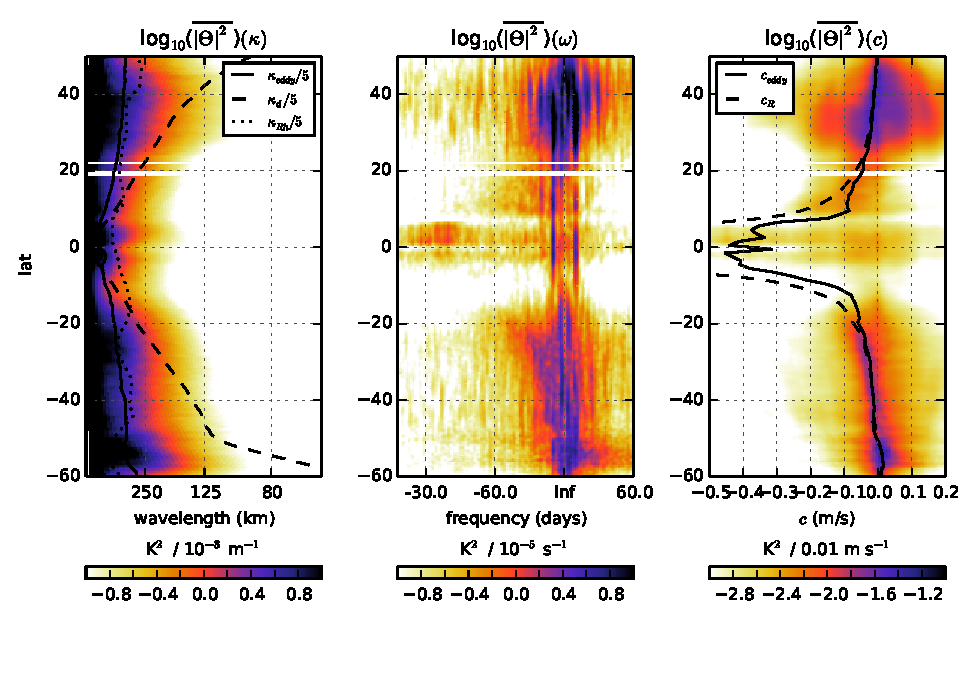
\includegraphics{../figures/SAT_50degwide/integrated_spectra_T.pdf}\\
  \caption{Power spectral density of SST variance as a function of latitude and inverse wavelength (left), frequency (center), and phase speed(right). All color scales are logarithmic. In the left panel, the average tracked-eddy inverse wavelength ($K_{eddy}/2\pi$, from \citealt{CheltonEtAl2011}), the Rossby deformation inverse wavelength ($K_d/2\pi$, from \citealt{TullochEtAl2011}), and the Rhines inverse wavelength ($K_{\beta} / 2\pi$) are also plotted. In the right panel, the long Rossby wave phase speed ($c_R$) and the speed of tracked nonlinear eddies ($c_{eddy}$, from \citealt{CheltonEtAl2011}) are also plotted.}
  \label{fig:integrated_spectra_T}
\end{figure}

\begin{figure}[t]
  \noindent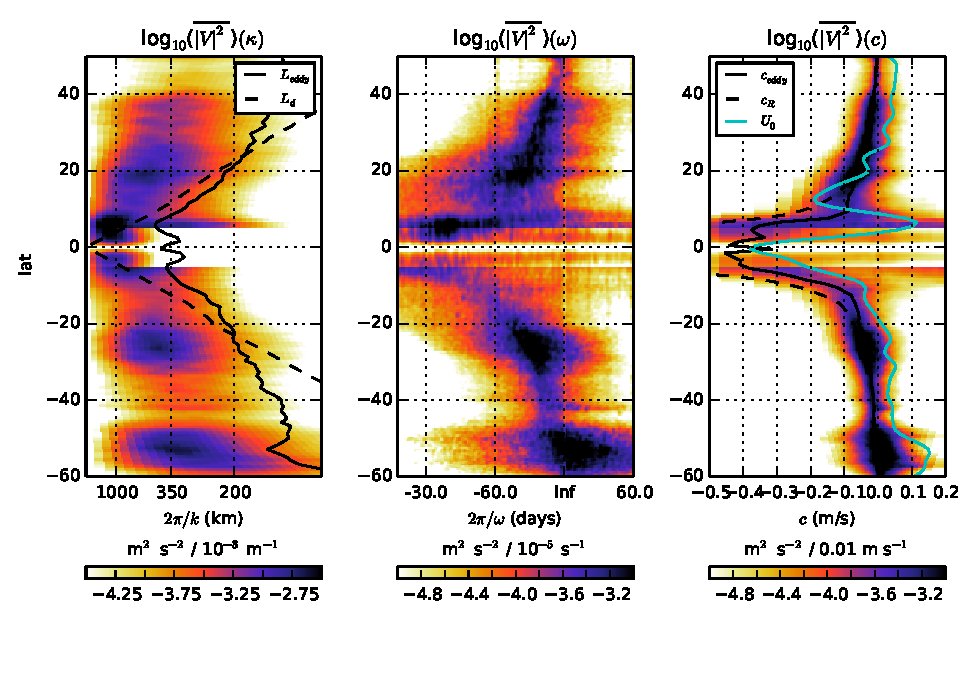
\includegraphics{../figures/SAT_50degwide/integrated_spectra_V.pdf}\\
  \caption{The same as Fig.~\ref{fig:integrated_spectra_T}, but for the SSH-derived meridional velocity.}
  \label{fig:integrated_spectra_V}
\end{figure}

\subsection{Eddy Heat Flux Cross Spectra}

Parseval's theorem also applies to the product of $\theta$ and $v$; the eddy heat flux is the same whether expressed as an average of space / time components or a sum of Fourier components. We express this mathematically as
\begin{equation}
\ol{V\Theta} = \frac{1}{MN} \sum_{m=0}^{M-1} \sum_{n=0}^{N-1} v_{mn} \theta_{mn} = \sum_{j=-\frac{M}{2}}^{\frac{M}{2}-1} \sum_{l=0}^{\frac{N}{2}-1} \Re \{ V_{jl}^\ast  \Theta_{jl} \} \ .
\end{equation}
Just as described above for the univariate spectra, we can sum the components of $\Re \{ V_{jl}^\ast  \Theta_{jl} \}$ selectively to define $\ol{V\Theta}(\varphi, k)$, $\ol{V\Theta}(\varphi, \omega)$, and $\ol{V\Theta}(\varphi, c)$. These functions are plotted in  Fig.~\ref{fig:integrated_spectra_VT}. Unlike the power spectra described above $\ol{V\Theta}$ can take both positive and negative values, corresponding to northward and southward heat transport. As seen in Fig.~\ref{fig:integrated_spectra_VT}, the eddy heat flux is poleward in both hemispheres, except near the equator, where it reverses. This is consistent with the mean SST gradient, which also reverses near the equator; the eddy flux is always down gradient. Further discussion and comparison of the spectra is deferred until Sec.~4.  %(The eddy diffusivity is discussed in Sec.~5).
%The spatial structure of the magnitude of the three $\ol{V\Theta}$ functions resembles that of $\ol{|V|^2}$ more than it does that of $\ol{|\Theta|^2}$. While $\ol{|\Theta|^2}(k)$ peaks at the lowest wavenumbers at every latitude, both  $\ol{|V|^2}(k)$ and $\ol{V\Theta}(k)$ peak at an intermediate wavenumber, presumably one associated with mesoscale eddies.

\begin{figure}[t]
  \noindent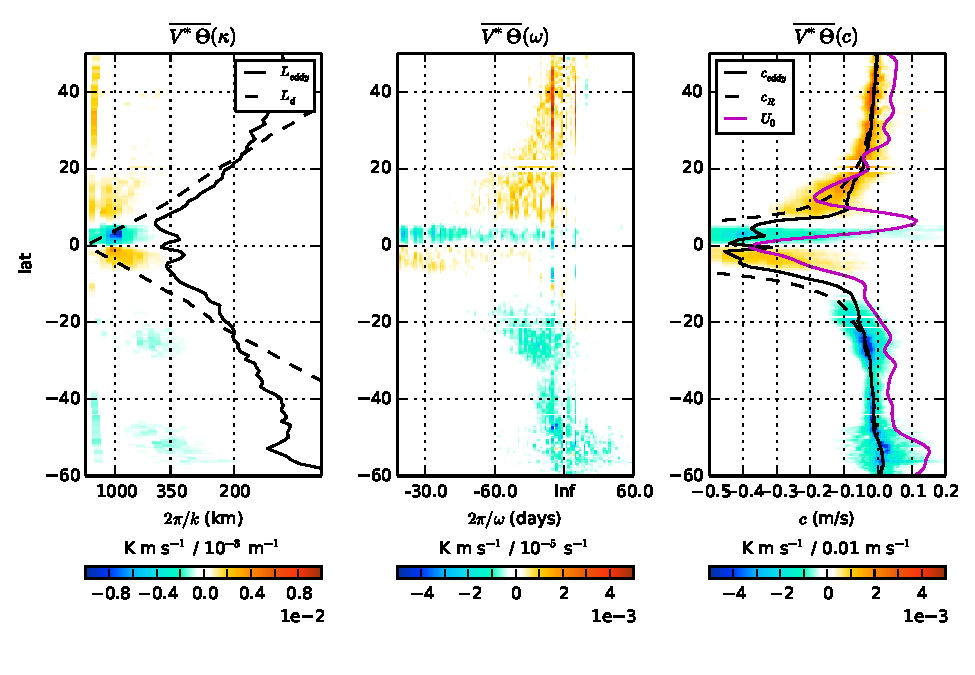
\includegraphics{../figures/SAT_50degwide/integrated_spectra_VT.pdf}\\
  \caption{Cross spectral density $\ol{V\Theta}$  as a function of latitude and wavelength (left), frequency (center), and phase speed(right). Otherwise the same as Fig.~\ref{fig:integrated_spectra_T}.}
  \label{fig:integrated_spectra_VT}
\end{figure}

\subsection{Cross-Spectral Analysis of 1/10$^\circ$ POP Model}

The analysis of the model is identical. Only the spatiotemporal sampling and resolution are different. For the model $L$, the sector width is the same, $N = 500$, $T=1825$ days, and $M=1825$. The different spectra from the POP model are shown in Figs.~\ref{fig:integrated_spectra_T_POP}, \ref{fig:integrated_spectra_V_POP}, and \ref{fig:integrated_spectra_VT_POP}.

\begin{figure}[t]
  \noindent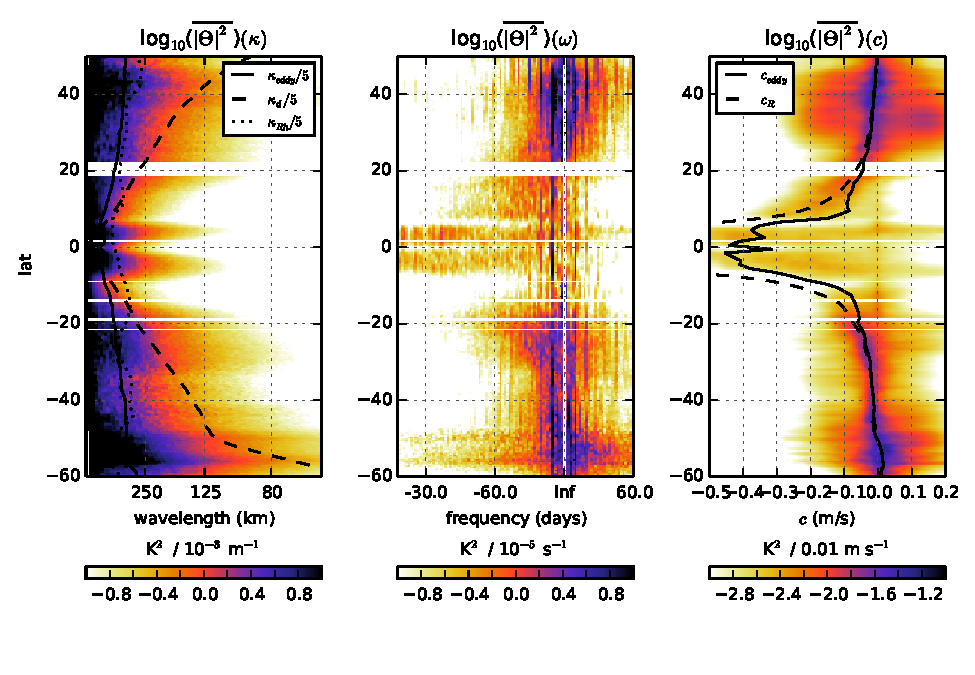
\includegraphics{../figures/POP_50degwide/integrated_spectra_T.pdf}\\
  \caption{The same as Fig.~\ref{fig:integrated_spectra_T}, but for the POP model SSH.}
  \label{fig:integrated_spectra_T_POP}
\end{figure}

\begin{figure}[t]
  \noindent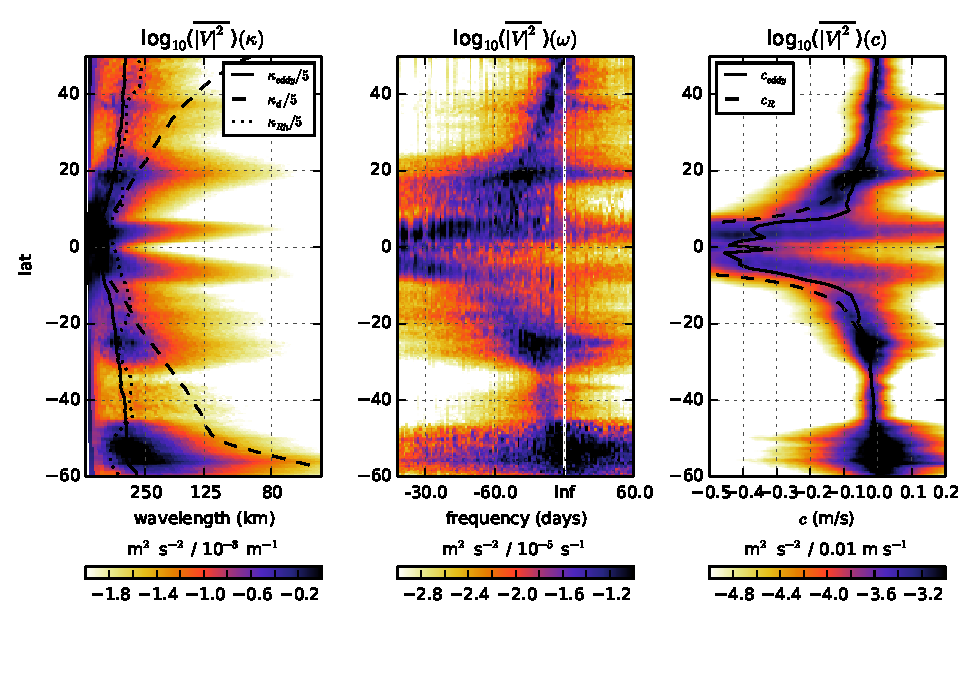
\includegraphics{../figures/POP_50degwide/integrated_spectra_V.pdf}\\
  \caption{The same as Fig.~\ref{fig:integrated_spectra_V}, but for the POP model surface meridional velocity.}
  \label{fig:integrated_spectra_V_POP}
\end{figure}

\begin{figure}[t]
  \noindent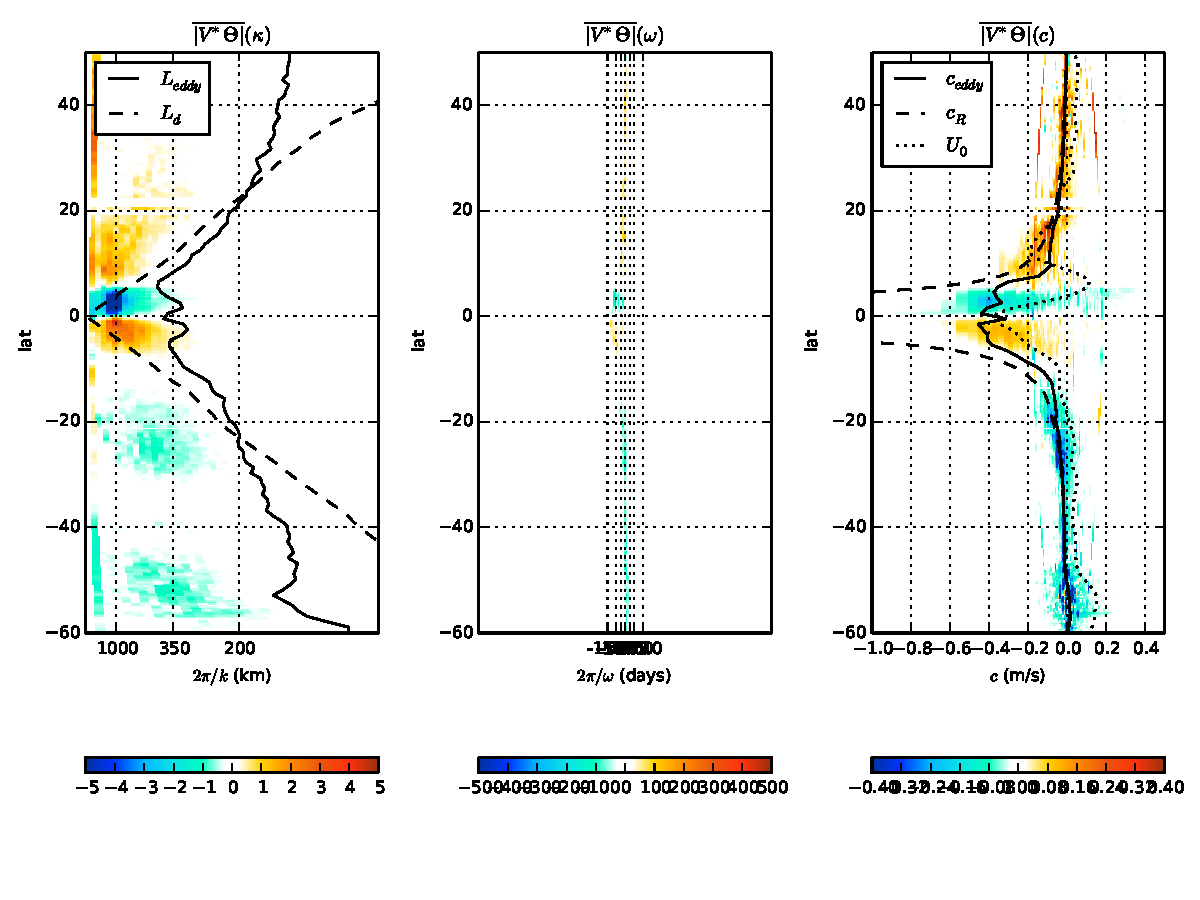
\includegraphics{../figures/POP_50degwide/integrated_spectra_VT.pdf}\\
  \caption{The same as Fig.~\ref{fig:integrated_spectra_VT}, but for the POP model surface meridional temperature flux.}
  \label{fig:integrated_spectra_VT_POP}
\end{figure}


\section{Spectral Moments and Discussion}

While a visual comparison of the spectra in Figs.~1-6 is informative, a more quantitative comparison is desirable. In particular, we wish to asses whether the spectra peak in the same locations and how those peaks are related to the underlying dynamics. Furthermore, we wish to assess to what extent the spectra are narrowly concentrated around these peaks, versus broadly distributed. In this section we characterize the properties of the power spectra and cross spectra via their moments in wavenumber, frequency, and phase speed space. The first moment tells us about the dominant scale. The second moment tells us how concentrated the distribution is about that scale. Spectral moments play an important role in the theory of geostrophic turbulence \citep[e.g.][]{Rhines1975}.

We define the first moment of a wavenumber spectrum $\ol{|\Theta|^2}(k)$ at a given latitude (itself defined in \ref{eq:Theta_kappa}) as
\begin{equation}
M^k_1 ( \ol{|\Theta|^2} ) = \frac{ \int k \ol{|\Theta|^2}(k) d k }{ \int \ol{|\Theta|^2}(k) d k }
\label{eq:M1}
\end{equation}
where the integrals are performed over all wavenumbers. The second moment is then defined as
\begin{equation}
M^k_2 (\ol{ |\Theta|^2 }) = \frac{ \int (k - M^1_k)^2 \ol{|\Theta|^2}(k) d k }{ \int \ol{|\Theta|^2}(k) d k } \ .
\label{eq:M2}
\end{equation}
We make analogous definitions for the $\omega$ and $c$ moments, and also for the moments of the other spectra $\ol{|V|^2}$ and $\ol{V \Theta}$. 

For a gaussian distribution, $M_1$ is the mean and $M_2$ is the variance. The interpretation of $M_1$ and $M_2$ is therefore most clear when the spectra have a clearly defined, dominant peak. In the case of $\ol{V \Theta}$,  which is not positive definite, it is possible for the normalization factor in the denominator of \eqref{eq:M1} and \eqref{eq:M2} to approach zero, leading to a meaningless result. To avoid this situation, we mask the moments at latitudes where the ratio $\int \ol{V\Theta} / \int | \ol{V \Theta} | < 0.9$. This is only the case in regions where the mean SST gradient is weak (primarily near 15$^\circ$S) and the heat flux is vanishingly small and noisy. At most latitudes, the heat flux does display a clear spectral peak, as evident in Figs.~\ref{fig:integrated_spectra_VT} and \ref{fig:integrated_spectra_VT_POP}.

The first moments $M_1^k( \ol{|\Theta|^2} )$, $M_1^k( \ol{|V|^2} )$, and $M_1^k( \ol{V \Theta} )$ are plotted in the upper panel Fig.~\ref{fig:moments_k}, with the second moments $M_2^k( \ol{|\Theta|^2} )$, $M_2^k( \ol{|V|^2} )$, and $M_2^k( \ol{V \Theta} )$ in the lower panel, for both the satellite data and the POP model. The $c$ moments are in shown in Fig.~\ref{fig:moments_c}. Equipped with this more quantitative description, we are now prepared to discuss the features and characteristics of the spectra.

\begin{figure}[t]
  \noindent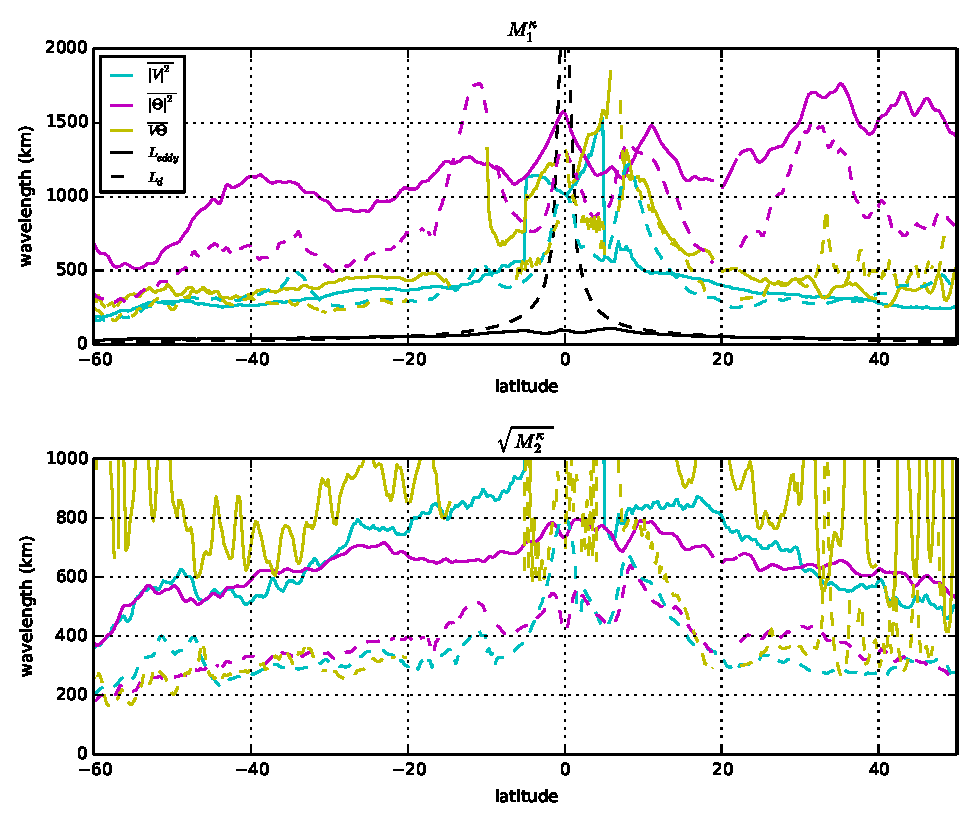
\includegraphics{../figures/moments_k.pdf}\\
  \caption{The first moments $M_1^k$ (upper panel) and second moments $M_2^k$ (middle panel) of the wavenumber spectra $\ol{|\Theta|^2}(k)$ (blue), $\ol{|V|^2}(k)$ (green), and $\ol{V\Theta}(k)$ (red). The satellite data are plotted with solid lines, and the POP model is plotted with dashed lines. In the upper panel the wavenumber has been converted to wavelength for plotting. The observed coherent eddy wavelength $L_{eddy}$ (solid black) and the deformation wavelength $L_d$ (dashed black) are also plotted. In the middle panel, the square root of the second moment is shown, indicating the ``width" of the spectra in $k$ space. In the bottom panel, the ratio between the observed coherent eddy wavenumber, the deformation wavenumber, and the Rhines wavenumber and $M_1^k(\ol{V\Theta}$ is shown; where this ratio is greater than 1, it means that the heat flux is dominated by scales {\em larger} than the comparison scale. }
  \label{fig:moments_k}
\end{figure}

\begin{figure}[t]
  \noindent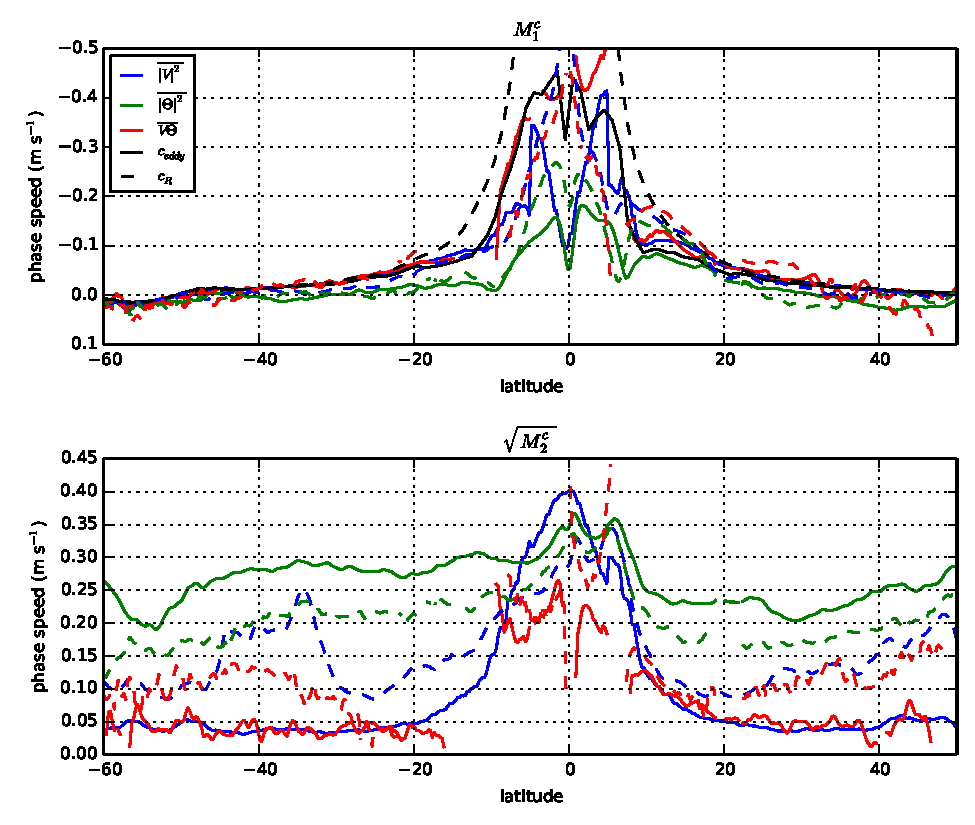
\includegraphics{../figures/moments_c.pdf}\\
  \caption{The same as Fig.~\ref{fig:moments_k}, but for the $c$-moments. In the upper panel, the tracked coherent eddy phase speed $c_{eddy}$ (solid black) and the long-wave Rossby wave phase speed from linear theory $c_R$ (dashed black) are also plotted. }
  \label{fig:moments_c}
\end{figure}

Regarding the lengths scales of the eddy heat flux $\ol{V\Theta}(k)$, is is noteworthy that at all latitudes it is concentrated at relatively low wavenumbers, corresponding to wavelengths of 250 km or greater (Fig.~\ref{fig:moments_k}). Generally speaking, these are the same wavelengths containing most of the kinetic energy (as indicated by $\ol{|V|^2}(k)$). The dominance of these wavelengths in the kinetic energy has been noted by other authors \citep[e.g.][]{Stammer1997,Wunsch2010,WorthamWunsch2014} and has been attributed to the work a geostrophic-turbulent inverse cascade of energy from some source scale to the deformation radius. It is interesting, although unsurprising, to see that these wavelengths also dominate the heat flux. (Unsurprising because large eddies are the most efficient at transporting tracers.) The consistent proportionality between the dominant length scale of the heat flux and the diameter of coherent mesoscale eddies strongly suggests that the mesoscale eddies are responsible for the heat transport. This conclusions stands somewhat in contrast to \citet{KillworthEtAl2004}, who attributed the large scales in ocean color / SSH cross spectra to advection by long linear Rossby waves.

Of course, when interpreting the wavenumber spectra, we must keep in mind the low-pass-filtering effect of the AVISO processing, which artificially attenuates small scales. In this respect, comparison with the POP results is illuminating. It is clear from Figs.~1-6 that there is significantly more small-scale variance in the POP fields. This is reflected in larger values of $M_2^k$ (Fig.~\ref{fig:moments_k}) for the POP model by a factor of 2-3 for all three spectra. The values of $M_1^k(\ol{|\Theta|^2})$ are are also significantly different between the POP model and the data; a shift to shorter wavelengths is seen in the model SST. Since the SST spectra are red throughout (in contrast the energy spectra, which are peaked), this shift is expected from the resolution of smaller scales by the model. 

However, given the overall redness of the ocean energy spectrum, and the fact that the observations do resolve the most energetic scales well, we feel the above conclusions are robust.

\citet{KeatingSmith}


\section{Net Meridional Heat Transport and Eddy Diffusivity}

Finally, to put these results in the context of global climate, we calculate the net meridional eddy heat transport from both the satellite data and POP model. This heat transport is defined as
\begin{equation}
\mathcal{H} = \rho_0 c_p h \ol{v'\theta'}
\label{eq:H}
\end{equation}
where $\rho_0 = 1027$ kg m$^{-3}$ is a reference density and $c_p = 4186$ J K$^{-1}$ kg$^{-1}$ is the specific heat of seawater. In order to translate the surface eddy temperature flux $\ol{v'\theta'}$ into a heat flux, it must be multiplied by a finite depth $h$. This choice of depth strongly influences our estimate of $\mathcal{H}$. We opt for a conservative, lower bound estimate.

We can expect by definition that the observed surface velocities and temperatures are representative of the mixed layer. There can still be significant heat transport below the mixed layer which is likely well correlated with our surface estimate. Observational studies have shown the the vertical amplitude of eddy heat transport in the subtropical North Pacific is maximum near the surface and decays to zero over a depth scale of several hundred meters \citep{RoemmichGilson2001,QiuChen2005}. Since our surface observations cannot asses the subsurface component with any confidence, we simply present them as a lower bound on the vertically integrated heat transport. Based on the Argo-derived mixed-layer estimates of this sector from \citet{HolteTalley2009}, we use a spatially constant value of $h = 50$ m in \eqref{eq:H}. This is itself a lower bound; in the Southern Ocean, the annual mean mixed layer is considerably deeper. Furthermore, mixed layer depth exhibits considerable temporal variability. However, a spatially constant value facilities direct comparison between the model and the data, which is more important here than the precise magnitude of $\mathcal{H}$.

The value of $\mathcal{H}$ is shown in Fig.~\ref{fig:H}a for both satellite data and POP model, normalized to give units of TW (10$^{12}$ W) per degree of longitude. The order of magnitude in the extra-tropics is roughly 0.1 - 0.3 TW per degree, which scaled up to the width of the entire Pacific (over 100 degrees longitude), and accounting for some additional fraction of heat transport at depth, agrees generally with other global estimates \citep{JayneMarotzke2002,VolkovEtAl2008,DongEtAl2014}. 

The model and data agree generally quite well, both in spatial structure and magnitude of $\mathcal{H}$. Disagreement in magnitude, by factors of 2-3, arises in two principal locations: near the equator and in the ACC. (This disagreement is also visible, though not quite as obvious, in comparing Figs.~\ref{fig:integrated_spectra_VT} and \ref{fig:integrated_spectra_VT_POP} .) In these areas, the model produces a large eddy greater heat transport. What is the source of this disagreement? It is not simply that the model is ``wrong,'' since the observations themselves do not resolve the flux perfectly. Instead, seek to understand the physical reasons behind these differences.

KA14 argued, using kinematic simulations of passive tracer advection, that the eddy flux depends on four principal factors: the background meridional gradient, the eddy kinetic energy (EKE), the eddy size, and the eddy phase speed relative to the mean flow. While we do not attempt to quantitatively match their model here, it is instructive to consider these different factors when comparing the model with the data. Figs.~\ref{fig:moments_k} and \ref{fig:moments_c} suggest that the dominant length scales and phase speeds in the model and data are very similar. Therefore, we can expect the differences in $\mathcal{H}$ to be due to differences in background meridional gradient and eddy kinetic energy. 

In Fig.~\ref{fig:H}b, we plot the time and zonal mean meridional SST gradient $\partial \ol{\theta} /\partial \varphi$ from the model and the data. We see that the gradients are nearly identical, except in the equatorial region, where the model gradients can be 50\% larger. This partly explains the fact that the model $\mathcal{H}$ is higher in this region. The EKE, defined as $0.5 ( \ol{v'^2} + \ol{u'^2} )$, is plotted in Fig.~\ref{fig:H}c. (Technically only $v'$ enters directly in the meridional flux, but the eddy velocities are relatively isotropic in the extratropics.) The model and data EKE are quite similar in the extratropics, but differ significantly at low latitudes and in the ACC. The model is uniformly more energetic, by a factor of 2 in the ACC at the equator, and the regions of EKE mismatch are the same as those of differing eddy heat flux. Therefore, we can also attribute the some of the discrepancy in heat transport to the discrepancy in EKE.

Finally, we plot the surface eddy diffusivity for heat, defined as
\begin{equation}
K = - \ol{v'\theta'} \big / \pd{\ol{\theta}}{\varphi} \ .
\end{equation}
Where the gradient vanishes, $K$ becomes singular. To avoid this, we mask $K$ wherever the absolute value of the gradient is less than one tenth of its global mean value. This occurs in different locations for model and data, making a direct comparison in the equatorial region difficult. Nevertheless, the differences observed in EKE are clearly reflected in $K$ as well. Moreover, the general pattern in $K$, low at high latitudes and high at low latitudes, is very consistent with KA14. That study examined the eddy diffusivity of a synthetic passive tracer advected by the AVISO velocity fields. The similarity in magnitude and spatial structure between this study and that one suggests that the eddy heat flux is generated kinematically through advection of the mean SST gradient by the geostrophic eddy field.

\begin{figure*}[t!]
  \noindent 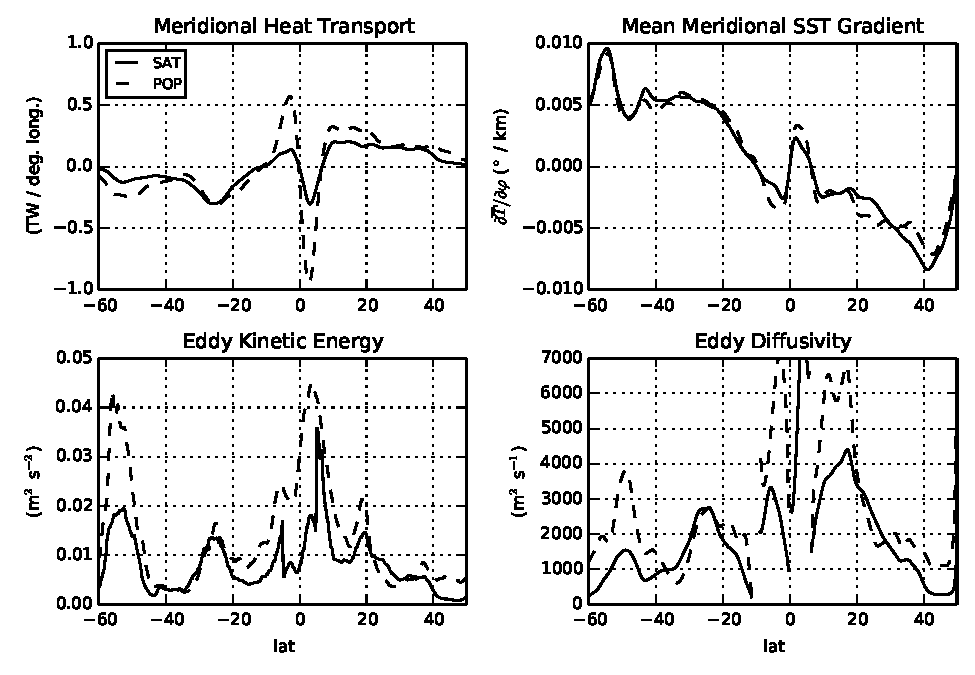
\includegraphics{../figures/MHT_gradient_EKE_diffusivity.pdf}\\
  \caption{Blah.}
  \label{fig:H}
\end{figure*}

\section{Conclusions}

The fact that the scales of eddy heat transport are so large suggests an alternative to the traditional diffusive parameterization of eddy fluxes in coarse-resolution models. 


Atmospheric waves propagate meridionally, but this propagation is constrained by their phase speed: they break when they encounter ``critical latitudes'' at which their phase speed matches the background mean flow. These dynamics leave a clear signature in atmospheric phase-speed cospecta \citep{ChenHeld2007}. Ocean eddies, in contrast, do not propagate far in latitude. However, we argue that the phase phase speed is still an important factor in understanding ocean eddy fluxes, since it plays a significant role in determining the eddy diffusivity \citep{AbernatheyEtAl2010,FerrariNikurashin2010}. In this study we show that the surface eddy heat flux at each latitude is relatively concentrated around the long-wave Rossby wave phase speed.


% a low frequency cutoff doesn't necessarily filter out non-mesoscale motions. Consider a stationary eddy in the ACC, propagating upstream but locked in place


% Use appendix}[A], {appendix}[B], etc. etc. in place of appendix if you have multiple appendixes.
\ifthenelse{\boolean{dc}}
{}
{\clearpage}

% Create a bibliography directory and place your .bib file there.
% -REMOVE ALL DIRECTORY PATHS TO REFERENCE FILES BEFORE SUBMITTING TO THE AMS FOR PEER REVIEW
\ifthenelse{\boolean{dc}}
{}
{\clearpage}
\bibliographystyle{ametsoc}
\bibliography{../bibliography/references}

%%%%%%%%%%%%%%%%%%%%%%%%%%%%%%%%%%%%%%%%%%%%%%%%%%%%%%%%%%%%%%%%%%%%%
% FIGURES-REMOVE ALL DIRECTORY PATHS TO FIGURE FILES BEFORE SUBMITTING TO THE AMS FOR PEER REVIEW
%%%%%%%%%%%%%%%%%%%%%%%%%%%%%%%%%%%%%%%%%%%%%%%%%%%%%%%%%%%%%%%%%%%%%
%\begin{figure}[t]
%  \noindent\includegraphics[width=19pc,angle=0]{figure01.pdf}\\
%  \caption{Enter the caption for your figure here.  Repeat as
%  necessary for each of your figures. Figure from \protect\cite{Knutti2008}.}\label{f1}
%\end{figure}
%%%%%%%%%%%%%%%%%%%%%%%%%%%%%%%%%%%%%%%%%%%%%%%%%%%%%%%%%%%%%%%%%%%%%
% TABLES
%%%%%%%%%%%%%%%%%%%%%%%%%%%%%%%%%%%%%%%%%%%%%%%%%%%%%%%%%%%%%%%%%%%%%
%\begin{table}[t]
%\caption{This is a sample table caption and table layout.  Enter as many tables as
%  necessary at the end of your manuscript. Table from Lorenz (1963).}\label{t1}
%\begin{center}
%\begin{tabular}{ccccrrcrc}
%\hline\hline
%$N$ & $X$ & $Y$ & $Z$\\
%\hline
% 0000 & 0000 & 0010 & 0000 \\
% 0005 & 0004 & 0012 & 0000 \\
% 0010 & 0009 & 0020 & 0000 \\
% 0015 & 0016 & 0036 & 0002 \\
% 0020 & 0030 & 0066 & 0007 \\
% 0025 & 0054 & 0115 & 0024 \\
%\hline
%\end{tabular}
%\end{center}
%\end{table}
%
\end{document}
